\RequirePackage{fix-cm}
\documentclass[12pt, oneside]{report}
\usepackage{scrextend}
\usepackage{mathptmx}
\DeclareMathAlphabet{\mathcal}{OMS}{cmsy}{m}{n}
\changefontsizes{13pt}
\usepackage[utf8]{vietnam}
\usepackage{tikz, pgf} 
\usetikzlibrary{patterns}
\usetikzlibrary{calc}
\usepackage{float}
\usepackage{lipsum}
\usepackage{longtable}

\usepackage{imakeidx} 
\makeatletter
\renewcommand\subitem{\@idxitem\nobreak\hspace*{10\p@}}
\renewcommand\subsubitem{\@idxitem\nobreak\hspace*{10\p@}\@idxsubitem\nobreak\hspace*{10\p@}}
\makeatother
\makeindex

\usepackage[left=3.50cm, right=2cm, top=3.50cm, bottom=3.0cm, a4paper]{geometry}
\usepackage{graphicx}
\usepackage{amsmath}
\usepackage{indentfirst}
\usepackage{booktabs}
\usepackage{amssymb}
\usepackage{multirow}
\usepackage{float}
\usepackage{amsthm}
\usepackage{subcaption}
\usepackage[unicode]{hyperref}
\renewcommand{\baselinestretch}{1.5}
\usepackage{enumitem}
\newcommand{\scaler}{0.7}
\graphicspath{ {figures/} }
\usepackage{array}
\usepackage{url}
\usepackage{adjustbox}

% Source code formatting for C++
\usepackage{listings}
\usepackage{xcolor}
\definecolor{codegreen}{rgb}{0.0,0.5,0.0}
\definecolor{codegray}{rgb}{0.5,0.5,0.5}
\definecolor{codepurple}{rgb}{0.58,0,0.82}
\definecolor{codeblue}{rgb}{0.0,0.0,0.7}
\definecolor{backcolour}{rgb}{0.96,0.96,0.96}
\lstdefinestyle{cppstyle}{
    backgroundcolor=\color{backcolour},
    commentstyle=\color{codegreen},
    keywordstyle=\color{codeblue}\bfseries,
    numberstyle=\tiny\color{codegray},
    stringstyle=\color{codepurple},
    basicstyle=\ttfamily\footnotesize,
    breakatwhitespace=false,
    breaklines=true,
    captionpos=b,
    keepspaces=true,
    numbers=left,
    numbersep=6pt,
    showspaces=false,
    showstringspaces=false,
    showtabs=false,
    tabsize=2,
    frame=single,
    language=C++
}
\lstset{style=cppstyle}
\renewcommand{\lstlistingname}{Listing}
\renewcommand{\lstlistlistingname}{List of Listings}

\hypersetup{colorlinks,linkcolor={black},citecolor={blue},urlcolor={red}}  \usepackage{multido}
\newcommand{\Pointilles}[1]{%
  \par\nobreak
  \noindent\rule{0pt}{1.5\baselineskip}%
  \multido{}{#1}{\noindent\makebox[\linewidth]{\dotfill}\endgraf}%
  \bigskip%
}

\newtheorem{dn}{Definition}[chapter]
\newtheorem{dl}{Theorem}[chapter]
\newtheorem{hq}{Corollary}[chapter]
\newtheorem{nx}{Remark}[chapter]
\newtheorem{vd}{Example}[section]
\renewcommand\qedsymbol{$\blacksquare$}

\newcommand\diag{\text{Diag}}
\DeclareMathOperator*{\argmax}{arg\,max}
\DeclareMathOperator*{\argmin}{arg\,min}
\usepackage[numbers,sort]{natbib}

\usepackage{algorithm}
\usepackage{algorithmic}
\usepackage{bm}
\usepackage{fancyhdr}

\usepackage{calc}
\makeatletter
\providecommand{\@address}{\textbackslash{}address\{\}}
\providecommand{\@title}{\textbackslash{}title\{\}}
\providecommand{\@reporttype}{\textbackslash{}reporttype\{\}}
\providecommand{\@major}{\textbackslash{}major\{\}}
\providecommand{\@specialize}{\textbackslash{}specialize\{\}}
\providecommand{\@author}{\textbackslash{}author\{\}}
\providecommand{\@date}{\textbackslash{}date\{\}}
\providecommand{\@school}{\textbackslash{}school\{\}}
\providecommand{\@supervisor}{\textbackslash{}supervisor\{\}}
\providecommand{\@class}{\textbackslash{}class\{\}}
\providecommand{\@email}{\textbackslash{}email\{\}}
\providecommand{\@studentid}{\textbackslash{}studentid\{\}}
\newcommand{\school}[1]{\def\@school{#1}}
\newcommand{\address}[1]{\def\@address{#1}}
\newcommand{\reporttype}[1]{\def\@reporttype{#1}}
\newcommand{\major}[1]{\def\@major{#1}}
\newcommand{\specialize}[1]{\def\@specialize{#1}}
\newcommand{\supervisor}[1]{\def\@supervisor{#1}}
\newcommand{\class}[1]{\def\@class{#1}}
\newcommand{\email}[1]{\def\@email{#1}}
\newcommand{\studentid}[1]{\def\@studentid{#1}}

\def\ttp@InsertUni{%
    \large%
    \expandafter\MakeUppercase{Hanoi University of Science and Technology}%
}
\def\ttp@InsertSchool{%
    \large
    \expandafter\MakeUppercase{Faculty of Information Technology}%
}

\def\ttp@InsertType{%
    \Large
    \expandafter\MakeUppercase{\@reporttype}%
}

\def\ttp@InsertDate{%
    \normalsize%
    {\@address\vspace{0.1cm} -- \@date}%
}

\def\ttp@InsertTitle{%
    \Large%
    \@title%
}

\def\ttp@InsertAuthor{%
    \large%
   \@author%
}

\def\majorname{Major:}
%\def\specializename{Chuyên sâu:}
\def\ttp@InsertMajor{%
    \large
    \majorname{} \@major\\%
    %\specializename{} \@specialize%
}

\def\ttp@InsertEmail{%
    \large
    \textnormal{\texttt{\@email}}%
}


\def\maketitle{%
\savegeometry{geo}%
\begin{titlepage}%
\bfseries\centering%
{\ttp@InsertUni}%
\\
{\ttp@InsertSchool}\\
{\Large
% \hrule height 1pt depth 0.5ex width 4cm \relax%
\begin{tikzpicture}
\draw[line width=2pt] (0ex,0ex) (0, 0.25ex) -- (4, 0.25ex);
\end{tikzpicture}%
\kern-0.1ex\relax{}o0o\kern-0.1ex\relax
\begin{tikzpicture}
\draw[line width=2pt] (0ex,0ex) (0, 0.25ex) -- (4, 0.25ex);
\end{tikzpicture}%
% \begin{tikzpicture}[height=1ex]
% \draw[line width=2pt] (0, 0.5ex) -- (4, 0.5ex);
% \end{tikzpicture}o0o%
}
\vfill
{
\includegraphics[width =3cm]{694px-Logo_Hust.png}}
\par\bigskip
{\ttp@InsertAuthor\\ \ttp@InsertEmail}\\
\par\bigskip~\par\bigskip
{\ttp@InsertTitle}
\par\bigskip~\par\bigskip
{\ttp@InsertType}
\par
{\ttp@InsertMajor}
\par\bigskip~\par\bigskip~\par\bigskip
\vfill
\ttp@InsertDate
\end{titlepage}%
\loadgeometry{geo}}

\def\makesubtitle{%
\savegeometry{geo}%
\begin{titlepage}%
\centering
\bfseries
{\ttp@InsertUni}
\\
{\ttp@InsertSchool}\\
{\Large
% \hrule height 1pt depth 0.5ex width 4cm \relax%
\begin{tikzpicture}
\draw[line width=2pt] (0ex,0ex) (0, 0.25ex) -- (4, 0.25ex);
\end{tikzpicture}%
\kern-0.1ex\relax{}o0o\kern-0.1ex\relax
\begin{tikzpicture}
\draw[line width=2pt] (0ex,0ex) (0, 0.25ex) -- (4, 0.25ex);
\end{tikzpicture}%
% \begin{tikzpicture}[height=1ex]
% \draw[line width=2pt] (0, 0.5ex) -- (4, 0.5ex);
% \end{tikzpicture}o0o%
}
\vfill
{
\includegraphics[width =3cm]{694px-Logo_Hust.png}}
\par\bigskip~\par\bigskip
{\ttp@InsertTitle}
\par\bigskip~\par\bigskip
{\ttp@InsertType}
\par
%\bigskip
{\ttp@InsertMajor}
\par\bigskip~\par\bigskip~\par\bigskip
\begin{tabular}{ll}
    \multicolumn{2}{l}{\textbf{Supervisor:} \textnormal{\@supervisor}}\\
    \noalign{\bigskip}
    \multicolumn{2}{l}{\textbf{Group members:}}\\
    \noalign{\smallskip}
    \quad Mai Nam Khanh \textit{(Leader)} & \textnormal{1695177}\\
    \quad Hoang Le Anh Duc & \textnormal{1708098}\\
    \quad Vu Duy Tuan & \textnormal{1694599}\\
    \quad Pham Duc Tri & \textnormal{1694589}\\
\end{tabular}%
\par\bigskip~\par\bigskip
\vfill
{\ttp@InsertDate}
\end{titlepage}%
\loadgeometry{geo}}
\makeatother
\title{DESIGN AND IMPLEMENTATION OF A FINANCIAL TRANSACTION MANAGEMENT \& AUDIT SYSTEM USING OBJECT-ORIENTED PROGRAMMING}
\reporttype{TERM PROJECT REPORT}
\major{Information Technology}
\author{Mai Nam Khanh}
\address{HANOI}
\date{2026}
\school{Information Technology}
\supervisor{[Supervisor Name]}
\class{TROY CS22A - K68}
\email{khanh.mn@sis.hust.edu.vn}
\specialize{Information Technology}
\studentid{1695177}

% English caption labels (override vietnam package defaults)
\renewcommand{\figurename}{Figure}
\renewcommand{\tablename}{Table}
\renewcommand{\chaptername}{Chapter}

\begin{document}
\renewcommand{\figurename}{Figure}
\renewcommand{\tablename}{Table}
\renewcommand{\chaptername}{Chapter}

\maketitle
\makesubtitle

\newpage
\thispagestyle{empty}
\newgeometry{left=2.5cm,right=2.8cm,top=2cm,bottom=2cm}
\setcounter{page}{1}

\fontsize{13pt}{16pt}\selectfont
\bigbreak
\begin{center}
	{\bfseries SUPERVISOR'S COMMENTS}
\end{center}
\bigbreak
\fontsize{13pt}{16pt}\selectfont
\bigbreak
\begin{enumerate}
	\item [{\bfseries 1.}]{\bfseries Objectives and content of the project}
            \vspace{5cm}
	\item [{\bfseries 2.}] {\bfseries Achieved results}
            \vspace{5cm}
	\item [{\bfseries 3.}]{\bfseries Students' working attitude}
            \vspace{5cm}
\end{enumerate}
\hspace{0.5\textwidth}
\begin{minipage}{0.5\textwidth}
	\noindent\begin{center}
		\textit{Hanoi, \today} \\
		Supervisor\\ \vspace{2cm}
		\textbf{[Supervisor Name]}
	\end{center}	
\end{minipage}
\restoregeometry

\chapter*{Acknowledgement}
The group would like to express its sincere gratitude to the instructor of the Object-Oriented Programming course, who has devotedly imparted fundamental knowledge and guided the group throughout the implementation of this term project.

The lectures on object-oriented principles, together with valuable professional feedback, helped the group not only complete the product but also develop a systematic and scientific approach to software design. This is an important foundation that gives each member greater confidence on the path of study and future professional development.

During the implementation, due to limitations in time and knowledge, this report may contain shortcomings. The group sincerely looks forward to receiving comments from the instructor in order to improve the topic further.

The group sincerely thanks you!

\chapter*{Abstract}
This report presents the process of analysing, designing, and implementing a \textbf{Financial Transaction Management \& Audit System} in the C++ programming language, strictly following the principles of Object-Oriented Programming (OOP).

The system simulates a real-world banking problem: automatically scanning large volumes of transactions to detect signs of financial fraud such as money laundering and the splitting of cash flows (\textit{smurfing}). Architecturally, the system is divided into four independent functional modules and fully applies object-oriented techniques: abstraction through abstract classes and interfaces, single and multiple inheritance, polymorphism via dynamic dispatch, together with advanced memory-management techniques such as the Rule of Five and the Virtual Constructor idiom.

Experimental results show that the system operates stably, accurately detects violating transactions under several types of audit rules, is free of memory leaks, and clearly demonstrates extensibility -- a new audit rule can be added without modifying the core source code of the system.

\textbf{Keywords:} Object-Oriented Programming, C++, Polymorphism, Multiple Inheritance, Memory Management, Financial Fraud Detection.


\renewcommand{\contentsname}{Table of Contents}
\tableofcontents

\chapter*{List of Abbreviations}

\begin{tabular}{@{\hspace{-0.1cm}} l @{\hspace{1.2cm}}p{11.5cm}l}
    \textbf{OOP} & Object-Oriented Programming\\
    \textbf{UML} & Unified Modeling Language\\
    \textbf{AML} & Anti-Money Laundering\\
    \textbf{API} & Application Programming Interface\\
    \textbf{CSV} & Comma-Separated Values\\
    \textbf{POD} & Plain Old Data\\
    \textbf{SRP} & Single Responsibility Principle\\
    \textbf{OCP} & Open/Closed Principle\\
    \textbf{RAII} & Resource Acquisition Is Initialization\\
    \textbf{vptr} & Virtual Pointer\\
    \textbf{vtable} & Virtual Table\\
    \textbf{SWIFT} & Society for Worldwide Interbank Financial Telecommunication\\
    \textbf{OFAC} & Office of Foreign Assets Control\\
    \textbf{IDE} & Integrated Development Environment\\
\end{tabular}


\renewcommand{\listtablename}{List of Tables}
\renewcommand{\listfigurename}{List of Figures}
\listoftables
\listoffigures
\lstlistoflistings

\newpage
\pagestyle{fancy}
\rhead{\fontsize{10pt}{18pt} \selectfont Introduction}
\lhead{\fontsize{11pt}{18pt} \selectfont TERM PROJECT REPORT}
\cfoot{\fontsize{13pt}{18pt} \selectfont \thepage}
\chapter*{Introduction}
\addcontentsline{toc}{chapter}{Introduction}

In the context of a rapidly growing digital economy, the volume of financial transactions executed every day worldwide is enormous. Alongside this convenience comes an ever-increasing risk of financial fraud, particularly money laundering and the splitting of cash flows (\textit{smurfing}) used to evade monitoring thresholds. Manually inspecting every transaction is infeasible; therefore, the need to build automated software systems capable of scanning and detecting suspicious transactions has become urgent.

Such a system requires not only business-level accuracy but also a sound software architecture: easy to maintain and easy to extend as legal regulations change and new types of fraud emerge. This is an ideal setting in which to apply the principles of Object-Oriented Programming (OOP) -- a programming paradigm that helps model complex business entities as clear software objects with high reusability and extensibility.

Motivated by this reality, the group chose the topic ``Design and Implementation of a Financial Transaction Management \& Audit System using Object-Oriented Programming''. The objective is to design and implement an engine capable of managing accounts and transactions and automatically assessing the risk of each transaction based on a polymorphic set of audit rules, while fully and deeply demonstrating the object-oriented techniques studied in the course.

\newpage
The content of this report is organised into three chapters as follows:

\begin{itemize}
    \item \textbf{Chapter 1: Project Overview.} Presents the context of the financial fraud detection problem, the objectives and scope of the system, the functional requirements, and the tools and development environment used.
    \item \textbf{Chapter 2: Theoretical Background and System Design.} Introduces the fundamental principles of Object-Oriented Programming, then presents in detail the overall architecture of the system through a UML class diagram, clarifying the role of each module and how the OOP principles are applied to the design.
    \item \textbf{Chapter 3: Implementation and Evaluation.} Presents in detail the implementation of the core components, illustrated with source code, the experimental results of the system, the verification of memory management, and the division of work within the group.
\end{itemize}

\vspace{1cm}
\hspace{0.5\textwidth}
\begin{minipage}{0.5\textwidth}
	\noindent\begin{center}
		\vspace{0.5cm}
		\textit{Hanoi, \today} \\
		The group of students
	\end{center}	
\end{minipage}


\newpage
\pagestyle{fancy}
\rhead{\fontsize{10pt}{18pt} \selectfont \nouppercase{\leftmark}}
\lhead{\fontsize{11pt}{18pt} \selectfont TERM PROJECT REPORT}
\cfoot{\fontsize{13pt}{18pt} \selectfont \thepage}

\chapter{Project Overview}

\section{Background and Significance of the Problem}
    Modern financial systems process an enormous volume of transactions every day. In parallel, financial crimes have become increasingly sophisticated, causing significant economic damage and threatening the stability of the banking system. Among these crimes, \textbf{money laundering} is one of the most serious problems faced by financial institutions.

    To evade the supervision of regulatory authorities, criminals often use the technique of \textbf{splitting cash flows} (\textit{smurfing} or \textit{structuring}): instead of conducting one large, easily detectable transaction, they divide the amount into many small transactions below the mandatory reporting threshold. In addition, transactions involving individuals or organisations on a sanctions list, or transactions originating from high-risk geographical regions, are also warning signs that require close monitoring.

    Manual inspection is infeasible at large data scales. Therefore, financial institutions rely on \textbf{Anti-Money Laundering} (AML) software systems \cite{Chen2018AML} that can automatically scan all transactions and compare them against a set of business rules to detect suspicious cases.

\section{Objectives and Scope}
    \subsection{Objectives}
    The project aims to build a \textbf{transaction audit engine} that simulates a real-world AML monitoring process, with two parallel objectives:

    \begin{itemize}
        \item \textbf{Business objective:} The system is able to manage a portfolio of accounts and transactions, then automatically scan and detect violating transactions based on several types of audit rules (large amount, smurfing, sanctions list, geographical anomaly).
        \item \textbf{Technical objective:} To fully and correctly apply the principles of Object-Oriented Programming, building a software architecture with a high level of abstraction that is easy to maintain and especially \textbf{easy to extend} -- allowing new audit rules to be added without changing the core source code.
    \end{itemize}

    \subsection{Scope}
    Within the framework of a course term project, the system focuses on the core business-logic processing and the object-oriented architecture, operating on a command-line (console) interface. Input data is loaded from CSV files or entered directly by the user; audit results are displayed on screen and exported to a plain-text report file.

\section{System Requirements}
    Based on the term project specification, the system must satisfy the following requirements:

    \begin{enumerate}
        \item \textbf{Data stored in files:} Account and transaction data must be able to be read from and written to files.
        \item \textbf{Maximum use of OOP techniques:} The program must demonstrate fundamental principles such as Abstraction, Inheritance, and Polymorphism, along with several advanced techniques.
        \item \textbf{At least four object classes:} The system must have at least four classes; in practice, the group's system has about fourteen classes and structures.
        \item \textbf{Clear division of work:} Each member is responsible for a specific portion of the source code and participates in the coding process.
    \end{enumerate}

    \subsection{Main Functions}
    The system provides the following interactive functions for the user:
    \begin{itemize}
        \item Add a new account (a retail account or a corporate account).
        \item Add a new transaction (a domestic transfer or an international transfer).
        \item Display the list of existing accounts and transactions.
        \item Select audit rules and run the automatic scanning process.
        \item Export the audit result report to a file.
        \item Quickly load a sample data set from CSV files for demonstration.
    \end{itemize}

\section{Tools and Development Environment}
    The project was developed using the following environment and toolset:
    \begin{itemize}
        \item \textbf{Programming language:} C++, using the C++17 standard.
        \item \textbf{Compiler:} GCC (g++) via the w64devkit toolset on the Windows operating system.
        \item \textbf{Editor:} Visual Studio Code.
        \item \textbf{Version control:} Git and GitHub, applying a feature-branching model so that members can work in parallel.
        \item \textbf{Testing tool:} AddressSanitizer is used to verify memory management and ensure there are no leaks.
    \end{itemize}

    Using Git with a feature-branching model allows the four members of the group to work simultaneously on the four architectural modules (see Chapter 2). Each member develops on a separate branch (for example \texttt{feature/core-entities}, \texttt{feature/audit-rules}) and merges into the main branch through Pull Requests, which helps minimise source-code conflicts.

\chapter{Theoretical Background and System Design}

\section{Principles of Object-Oriented Programming}
    Object-Oriented Programming (OOP) is a programming paradigm based on the concept of an ``object'' -- an entity that contains both data (attributes) and behaviour (methods). OOP is built on four fundamental principles \cite{Stroustrup2013}, all of which are applied in the group's system.

    \subsection{Abstraction}
    Abstraction is the act of hiding complex implementation details and exposing only the essential characteristics of an object. In C++, abstraction is expressed through an \textbf{abstract class} containing \textbf{pure virtual functions}. An abstract class cannot be instantiated directly; it merely serves as a template for derived classes. In the system, the classes \texttt{Account}, \texttt{Transaction} and the interface \texttt{AuditRule} are all abstract classes.

    \subsection{Encapsulation}
    Encapsulation is the bundling of data and the methods that operate on that data into a single unit (a class), while controlling external access. C++ provides three access levels: \texttt{private}, \texttt{protected}, and \texttt{public}. In the system, sensitive attributes such as the account balance (\texttt{balance}) or the transaction amount (\texttt{amount}) are declared \texttt{protected} so that derived classes can inherit them while they remain hidden from the outside, and can only be accessed through \texttt{public} methods such as \texttt{getBalance()}.

    \subsection{Inheritance}
    Inheritance allows one class (the derived class) to reuse the attributes and methods of another class (the base class), expressing an ``is-a'' relationship. The system uses both forms of inheritance:
    \begin{itemize}
        \item \textbf{Single inheritance:} For example, \texttt{CorporateAccount} inherits from \texttt{Account}.
        \item \textbf{Multiple inheritance:} The class \texttt{InternationalTransfer} inherits simultaneously from \texttt{Transaction} and \texttt{ForeignExchange}, analysed in detail in Section~\ref{sec:multiple_inheritance}.
    \end{itemize}

    \subsection{Polymorphism}
    Polymorphism allows objects of different classes to respond to the same method call in different ways. In C++, runtime polymorphism is implemented through \textbf{virtual functions} and the \textbf{dynamic dispatch} mechanism. When a virtual method is called through a pointer or reference to the base class, the compiler relies on the \textbf{virtual table} (vtable) and the \textbf{virtual pointer} (vptr) to determine and call the correct version of the method of the derived class at run time.

    \begin{nx}
    It must be noted in particular that runtime polymorphism \textbf{only works when an object is accessed through a pointer or reference}. If a derived-class object is stored by value in a base-class variable, the \textit{object slicing} phenomenon occurs: the data specific to the derived class is cut off and the dynamic dispatch mechanism no longer takes effect. This is why the system consistently uses pointers (\texttt{Account*}, \texttt{Transaction*}, \texttt{AuditRule*}) in all data containers.
    \end{nx}

\section{Overall System Architecture}
    The system is designed following the Single Responsibility Principle (SRP) and the Open/Closed Principle (OCP) \cite{Martin2017}, and is divided into four independent functional modules. The overall UML class diagram of the system is presented in Figure~\ref{fig:uml_full}.

    \begin{figure}[H]
        \centering
        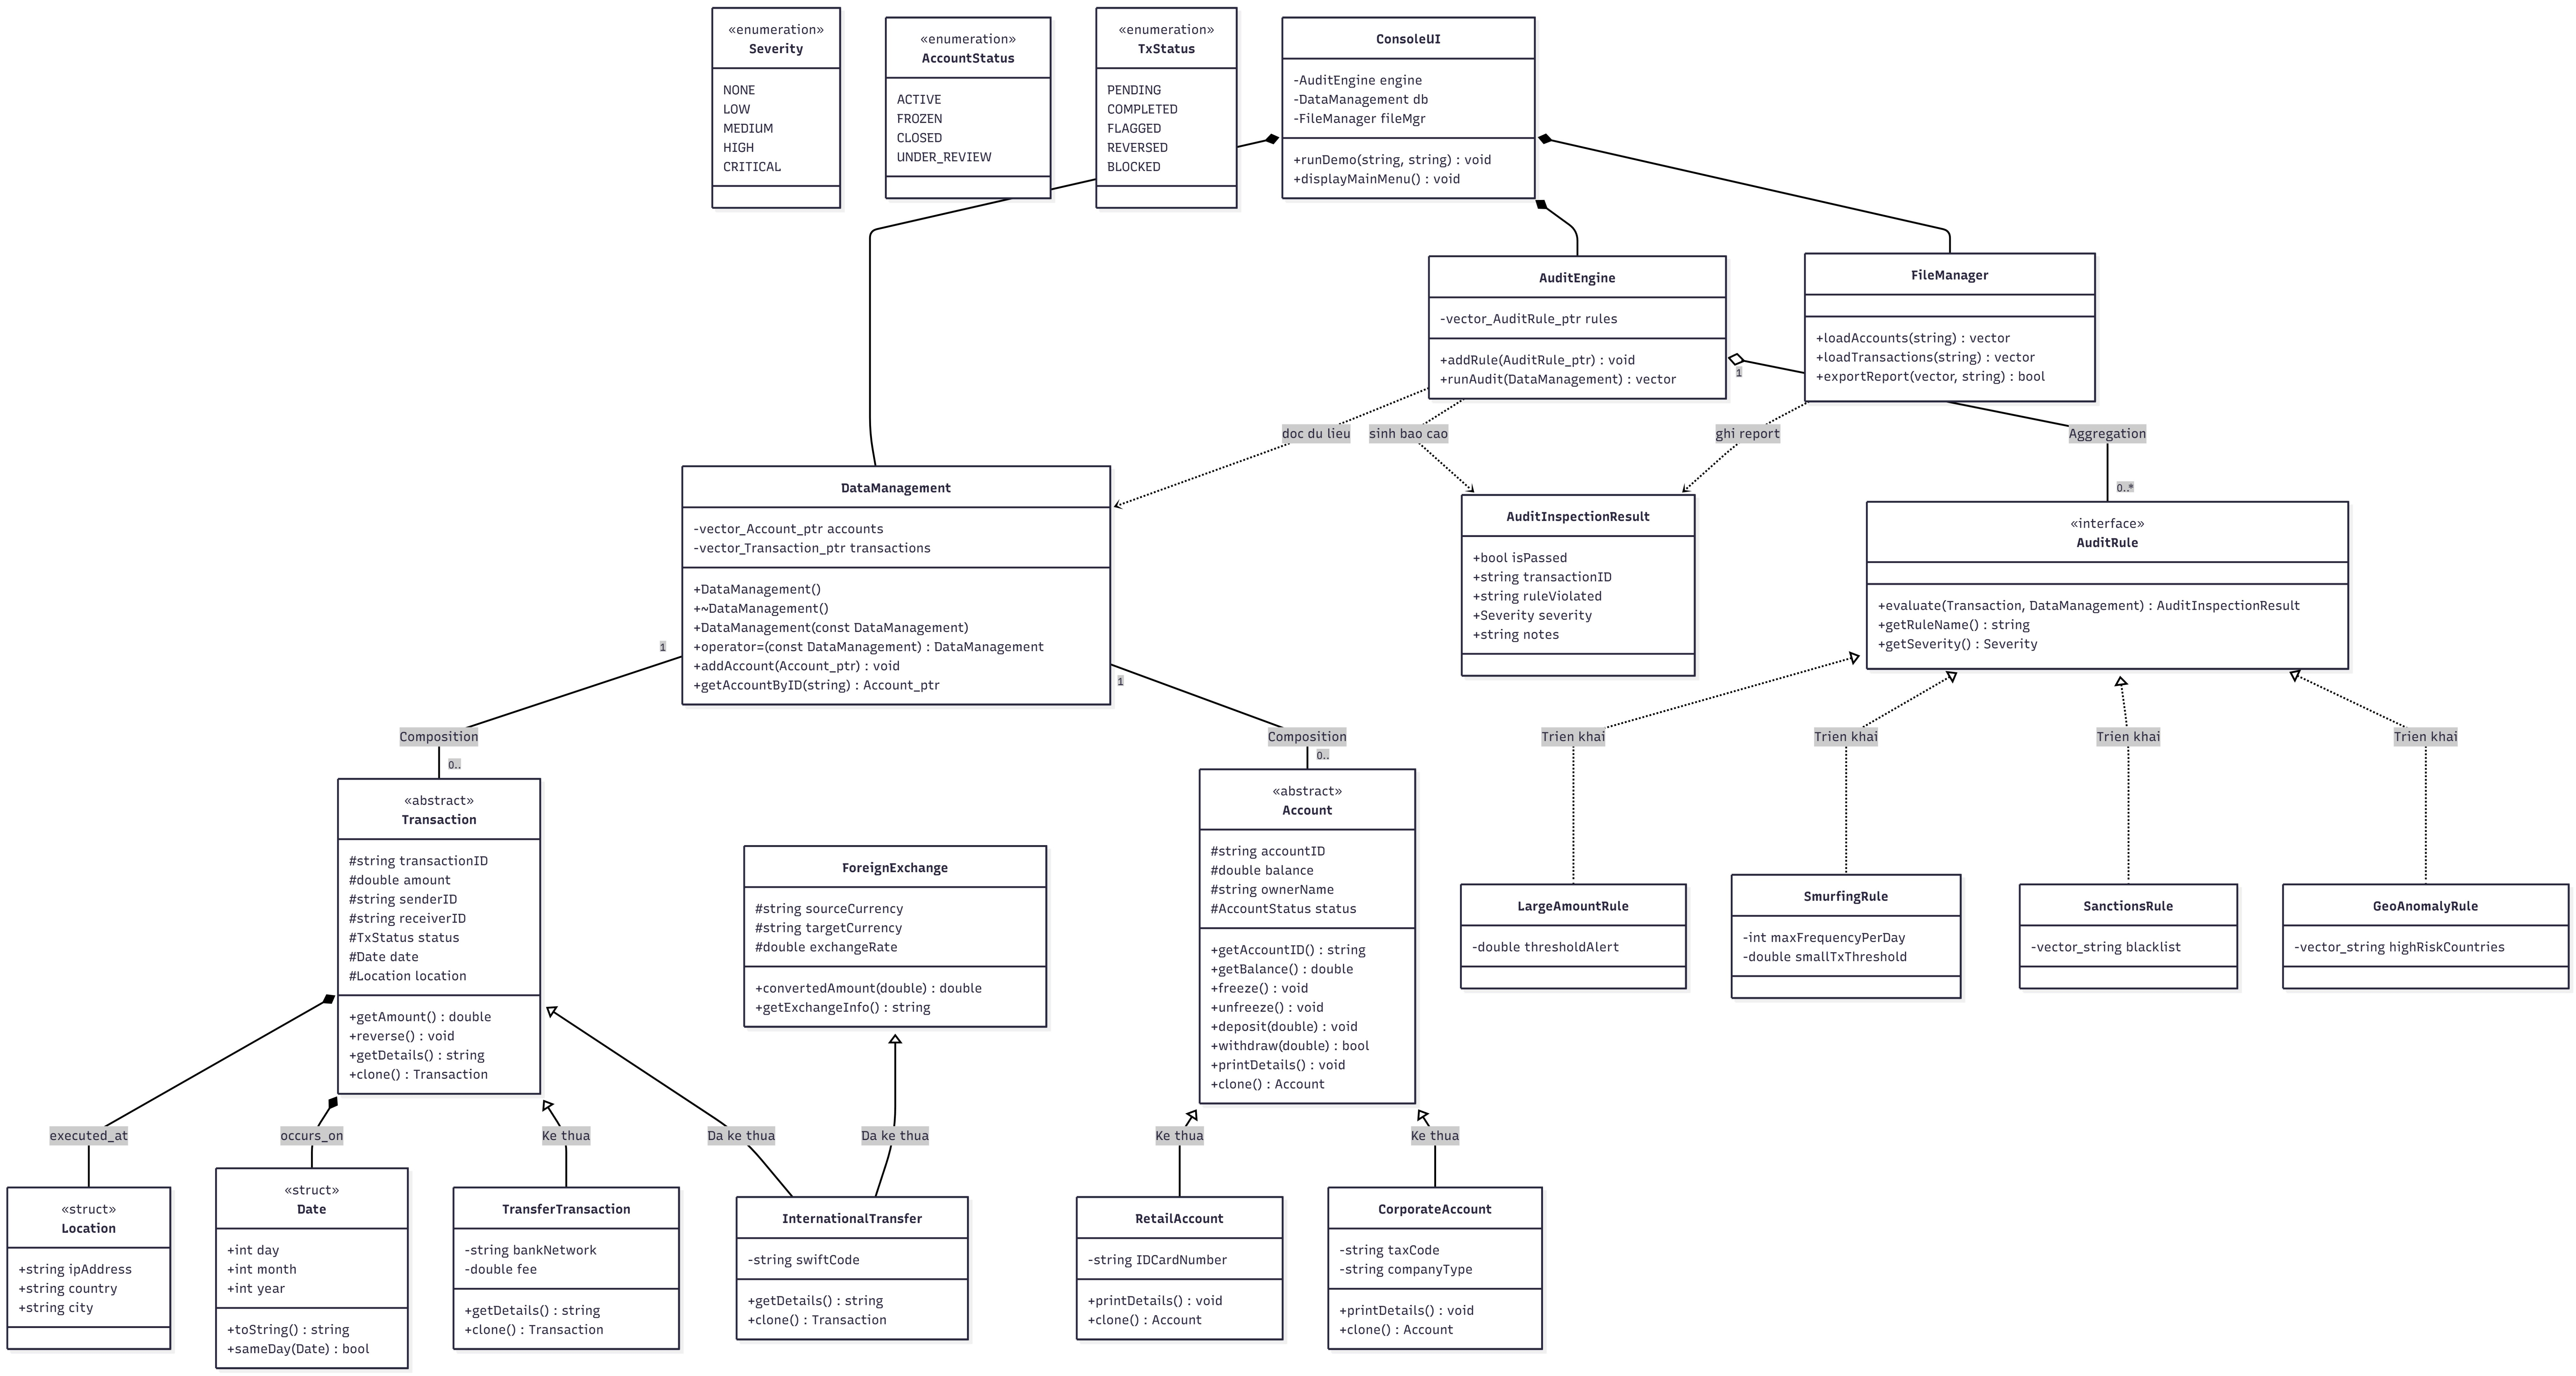
\includegraphics[width=\textwidth]{uml_full.png}
        \caption{Overall UML class diagram of the financial transaction management and audit system.}
        \label{fig:uml_full}
    \end{figure}

    The four functional modules are:
    \begin{itemize}
        \item \textbf{Data Structs module:} Contains Plain-Old-Data (POD) structs such as \texttt{Date}, \texttt{Location} and the enumeration types (\texttt{enum class}) \texttt{Severity}, \texttt{AccountStatus}, \texttt{TxStatus}.
        \item \textbf{Core Entities module:} Contains the classes \texttt{Account}, \texttt{Transaction} and their derived classes -- modelling the central business entities.
        \item \textbf{Audit Rules module:} Contains the \texttt{AuditRule} interface and the concrete rules -- where polymorphism and extensibility are most clearly demonstrated.
        \item \textbf{Engine \& IO module:} Contains the classes \texttt{DataManagement}, \texttt{AuditEngine}, \texttt{FileManager} and \texttt{ConsoleUI} -- responsible for orchestration, data management, and user interaction.
    \end{itemize}

\section{Design of the Core Entities Module}
    \subsection{Account Class Hierarchy}
    The \texttt{Account} class is an abstract class containing common \texttt{protected} attributes (account ID, balance, owner name, status) and a pure virtual function \texttt{printDetails()}. Two derived classes inherit from it:
    \begin{itemize}
        \item \texttt{CorporateAccount}: adds a tax code (\texttt{taxCode}) and a company type.
        \item \texttt{RetailAccount}: adds an identity card number (\texttt{IDCardNumber}).
    \end{itemize}
    The \texttt{Account} class has a \textbf{virtual destructor} to ensure correct memory release when deleting a derived-class object through a base-class pointer. In addition, realistic banking methods such as \texttt{freeze()} (freezing a suspicious account), \texttt{deposit()}, and \texttt{withdraw()} are also added to more closely reflect banking operations.

    \subsection{Transaction Class Hierarchy and Multiple Inheritance}
    \label{sec:multiple_inheritance}
    The \texttt{Transaction} class is also an abstract class containing the common information of a transaction and has a \textbf{composition} relationship with the two structs \texttt{Date} and \texttt{Location}. The derived class \texttt{TransferTransaction} models a domestic transfer.

    The technical highlight is the class \texttt{InternationalTransfer}, which models an international transfer. An international transfer \textbf{is a transaction} (it needs a transaction ID, amount, sender, receiver) and at the same time \textbf{carries foreign-exchange characteristics} (it needs the source currency, target currency, exchange rate). Therefore, the group designed this class to inherit simultaneously from two classes:
    \begin{itemize}
        \item \texttt{Transaction}: provides the attributes and behaviour of a transaction.
        \item \texttt{ForeignExchange}: provides currency-conversion capability through the \texttt{convertedAmount()} method.
    \end{itemize}

    \begin{nx}
    Since the two base classes \texttt{Transaction} and \texttt{ForeignExchange} \textbf{do not share a common ancestor}, the \textbf{Diamond Problem does not occur}. Therefore, the system \textbf{does not need to use virtual inheritance}. This is a deliberate design decision aimed at keeping the structure simple and efficient.
    \end{nx}

\section{Design of the Audit Rules Module -- The Heart of Polymorphism}
    This module most clearly demonstrates the power of polymorphism and the Open/Closed Principle. At its centre is the abstract interface \texttt{AuditRule}, which defines a pure virtual method \texttt{evaluate()}. Each concrete audit rule is a derived class that implements this method according to its own logic:
    \begin{itemize}
        \item \texttt{LargeAmountRule}: detects a transaction whose value exceeds a given threshold.
        \item \texttt{SmurfingRule}: detects the cash-flow-splitting behaviour -- many small transactions on the same day from the same account.
        \item \texttt{SanctionsRule}: checks the sender/receiver against a sanctions list.
        \item \texttt{GeoAnomalyRule}: detects transactions originating from high-risk countries, making use of the information in the \texttt{Location} struct.
    \end{itemize}

    \begin{nx}
    An important design observation: the \texttt{SmurfingRule} cannot draw a conclusion based on a single transaction alone, because the nature of splitting is the need to count the \textbf{frequency} of many transactions. Therefore, the \texttt{evaluate()} method is designed to also receive a reference to the entire data store (\texttt{DataManagement}), allowing each rule to access the historical context when needed. Rules that only need to examine a single transaction (such as \texttt{LargeAmountRule}) simply ignore this parameter. Unifying a single method signature for all rules is precisely the foundation that allows the polymorphism mechanism to operate smoothly.
    \end{nx}

    \subsection{Extensibility under the Open/Closed Principle}
    Thanks to this polymorphic design, to add a new audit rule, a programmer only needs to create a new derived class of \texttt{AuditRule} and implement the \texttt{evaluate()} method. There is \textbf{no need to modify} the source code of \texttt{AuditEngine} or any other core component. The system is ``closed for modification but open for extension'' -- exactly in the spirit of the OCP.

\section{Design of the Engine Module and Relationships Between Classes}
    \subsection{The AuditEngine Class and the Aggregation Relationship}
    The \texttt{AuditEngine} class holds a container of rule pointers \texttt{vector<AuditRule*>}. The scanning process is performed using two nested loops: for each transaction, \texttt{evaluate()} is called in turn on each rule. It is precisely at this call that the dynamic dispatch mechanism (vtable/vptr) automatically selects the correct rule version to execute.

    The relationship between \texttt{AuditEngine} and \texttt{AuditRule} is an \textbf{Aggregation} relationship: \texttt{AuditEngine} has references to the rules and uses them, but does \textbf{not own} their lifetime. The rule objects are created externally and passed into the engine via the \texttt{addRule()} method.

    \subsection{The DataManagement Class and the Composition Relationship}
    In contrast, the \texttt{DataManagement} class has a \textbf{Composition} relationship with \texttt{Account} and \texttt{Transaction}: it \textbf{fully owns} these objects and is responsible for releasing them in its destructor. Because this class manages dynamic memory, it is designed following the Rule of Five (presented in Chapter 3).

    \subsection{The FileManager and ConsoleUI Classes}
    \texttt{FileManager} is responsible for reading data from CSV files and writing the report to a text file, implementing the requirement of storing data in files. \texttt{ConsoleUI} acts as the interface layer, orchestrating the entire user-interaction flow and connecting the three components \texttt{DataManagement}, \texttt{AuditEngine}, and \texttt{FileManager} together.

\section{Summary of Applied OOP Techniques}
    Table~\ref{tab:oop_techniques} summarises the object-oriented techniques applied in the system together with their corresponding locations.

    \begin{table}[H]
        \centering
        \caption{Summary of OOP techniques applied in the system}
        \label{tab:oop_techniques}
        \begin{tabular}{|l|p{8cm}|}
            \hline
            \textbf{Technique} & \textbf{Location in the system} \\ \hline
            Abstraction & Abstract classes \texttt{Account}, \texttt{Transaction}; interface \texttt{AuditRule} \\ \hline
            Encapsulation & \texttt{protected}/\texttt{private} attributes accessed via getters \\ \hline
            Single inheritance & \texttt{CorporateAccount}, \texttt{RetailAccount} inherit \texttt{Account} \\ \hline
            Multiple inheritance & \texttt{InternationalTransfer} inherits \texttt{Transaction} and \texttt{ForeignExchange} \\ \hline
            Polymorphism & Virtual methods \texttt{evaluate()}, \texttt{printDetails()}, \texttt{getDetails()} \\ \hline
            Virtual destructor & In the base classes \texttt{Account}, \texttt{Transaction}, \texttt{AuditRule} \\ \hline
            Operator overloading & \texttt{operator=} (copy and move) in \texttt{DataManagement} \\ \hline
            Rule of Five & The \texttt{DataManagement} class managing dynamic memory \\ \hline
            Composition & \texttt{DataManagement} owns \texttt{Account}, \texttt{Transaction} \\ \hline
            Aggregation & \texttt{AuditEngine} references \texttt{AuditRule} \\ \hline
            Enumeration (enum class) & \texttt{Severity}, \texttt{AccountStatus}, \texttt{TxStatus} \\ \hline
        \end{tabular}
    \end{table}

\chapter{Implementation and Evaluation}

\section{Project Source-Code Structure}
    The project is organised into multiple separate files by module, corresponding to the group's Git branching model. Each class is split into a header file (\texttt{.h}) and an implementation file (\texttt{.cpp}), which reduces compilation dependencies and allows members to work in parallel. The directory structure and division of work are presented in Table~\ref{tab:phancong} at the end of this chapter.

\section{Implementation of the Core Entities Module}
    \subsection{The Abstract Account Class}
    Listing~\ref{lst:account} illustrates the declaration of the abstract class \texttt{Account}. The \texttt{protected} attributes, the virtual destructor, the two pure virtual functions \texttt{printDetails()} and \texttt{clone()}, together with the business methods, can be clearly seen.

\begin{lstlisting}[caption={Declaration of the abstract Account class}, label={lst:account}]
class Account {                       // <<abstract>>
protected:                            // protected for derived classes
    std::string   accountID;
    double        balance;
    std::string   ownerName;
    AccountStatus status;
public:
    Account(std::string id, std::string owner, double bal);
    virtual ~Account() = default;     // virtual destructor

    std::string   getAccountID() const;
    double        getBalance()   const;
    AccountStatus getStatus()    const;

    // realistic banking operations
    void freeze();
    void unfreeze();
    bool withdraw(double amt);

    virtual void     printDetails() const = 0;   // pure virtual
    virtual Account* clone()        const = 0;    // Virtual Constructor
};
\end{lstlisting}

    \subsection{Multiple Inheritance in InternationalTransfer}
    Listing~\ref{lst:intl} illustrates the multiple-inheritance syntax. The \texttt{InternationalTransfer} class inherits from both \texttt{Transaction} and \texttt{ForeignExchange}, and calls the constructors of both base classes in its initialiser list.

\begin{lstlisting}[caption={Multiple inheritance in InternationalTransfer}, label={lst:intl}]
// Multiple inheritance: Transaction + ForeignExchange
// The two bases share no ancestor -> NO virtual inheritance needed
class InternationalTransfer : public Transaction, public ForeignExchange {
    std::string swiftCode;
public:
    InternationalTransfer(std::string id, double amt, std::string from,
                          std::string to, Date d, Location loc,
                          std::string src, std::string tgt,
                          double rate, std::string swift)
        : Transaction(id, amt, from, to, d, loc),
          ForeignExchange(src, tgt, rate),
          swiftCode(swift) {}
    std::string  getDetails() const override;
    Transaction* clone()      const override;
};
\end{lstlisting}

\section{Implementation of the Audit Rules Module -- Polymorphism}
    \subsection{The AuditRule Interface}
    Listing~\ref{lst:auditrule} shows the abstract interface for all rules. Note that the \texttt{evaluate()} method receives a \texttt{const DataManagement\&} reference so that rules requiring historical context can access it.

\begin{lstlisting}[caption={The abstract AuditRule interface}, label={lst:auditrule}]
class AuditRule {                     // <<interface>>
public:
    virtual ~AuditRule() = default;
    // Receives the DB so pattern-based rules can access history
    virtual AuditInspectionResult evaluate(
        const Transaction* t,
        const DataManagement& db) const = 0;
    virtual std::string getRuleName() const = 0;
    virtual Severity    getSeverity() const = 0;
};
\end{lstlisting}

    \subsection{Implementation of the Smurfing Detection Rule}
    Listing~\ref{lst:smurfing} shows how \texttt{SmurfingRule} traverses the entire transaction history to count small transactions on the same day from the same sender -- which is only possible thanks to the \texttt{db} parameter.

\begin{lstlisting}[caption={Smurfing detection logic}, label={lst:smurfing}]
AuditInspectionResult SmurfingRule::evaluate(
        const Transaction* t, const DataManagement& db) const {
    AuditInspectionResult r; r.transactionID = t->getID();
    if (t->getAmount() >= smallTxThreshold) return r; // only small tx
    int count = 0;
    for (auto* o : db.getTransactions())
        if (o->getSenderID() == t->getSenderID()
            && o->getDate().sameDay(t->getDate())
            && o->getAmount() < smallTxThreshold) ++count;
    if (count >= maxFrequencyPerDay) {
        r.isPassed = false;
        r.ruleViolated = getRuleName();
        r.severity = getSeverity();
    }
    return r;
}
\end{lstlisting}

    \subsection{The Polymorphic Audit Loop}
    The heart of the system lies in the \texttt{runAudit()} method of \texttt{AuditEngine} (Listing~\ref{lst:runaudit}). The call \texttt{rule->evaluate(t, db)} is exactly where the dynamic dispatch mechanism takes effect: the same line of code executes different logic depending on the actual rule type.

\begin{lstlisting}[caption={The audit loop with dynamic dispatch}, label={lst:runaudit}]
std::vector<AuditInspectionResult>
AuditEngine::runAudit(const DataManagement& db) const {
    std::vector<AuditInspectionResult> out;
    for (auto* t : db.getTransactions())
        for (auto* rule : rules) {
            // DYNAMIC DISPATCH: choose the right rule via vtable
            AuditInspectionResult res = rule->evaluate(t, db);
            if (!res.isPassed) out.push_back(res);
        }
    return out;
}
\end{lstlisting}

\section{Memory Management -- The Rule of Five}
    Because \texttt{DataManagement} owns dynamically allocated pointers, it must define five special functions for safe memory management: the destructor, the copy constructor, the copy assignment operator, the move constructor, and the move assignment operator. The challenge is that when copying a \texttt{vector<Account*>}, copying only the pointers would make two objects point to the same memory region (a \textit{shallow copy}), leading to a double-free error.

    The solution is the \textbf{Virtual Constructor} idiom \cite{Gamma1994}: each derived class implements the virtual method \texttt{clone()} that returns a copy of the correct type of itself. Thanks to this, the copy constructor can perform a \textbf{polymorphic deep copy} as shown in Listing~\ref{lst:ruleof5}.

\begin{lstlisting}[caption={Polymorphic deep copy via clone()}, label={lst:ruleof5}]
void DataManagement::deepCopyFrom(const DataManagement& o) {
    for (auto* a : o.accounts)
        accounts.push_back(a->clone());      // copy as the derived type
    for (auto* t : o.transactions)
        transactions.push_back(t->clone());
}
DataManagement::~DataManagement() { freeAll(); }   // free everything
\end{lstlisting}

\section{Experimental Results}
    \subsection{Interactive Interface}
    The system provides an interactive menu that allows the user to enter data, view lists, select audit rules, and export reports. The menu also includes an integrated Help \& Guide option that explains the input format directly within the program. Figure~\ref{fig:menu} shows the main menu and the report-export operation.

    \begin{figure}[H]
        \centering
        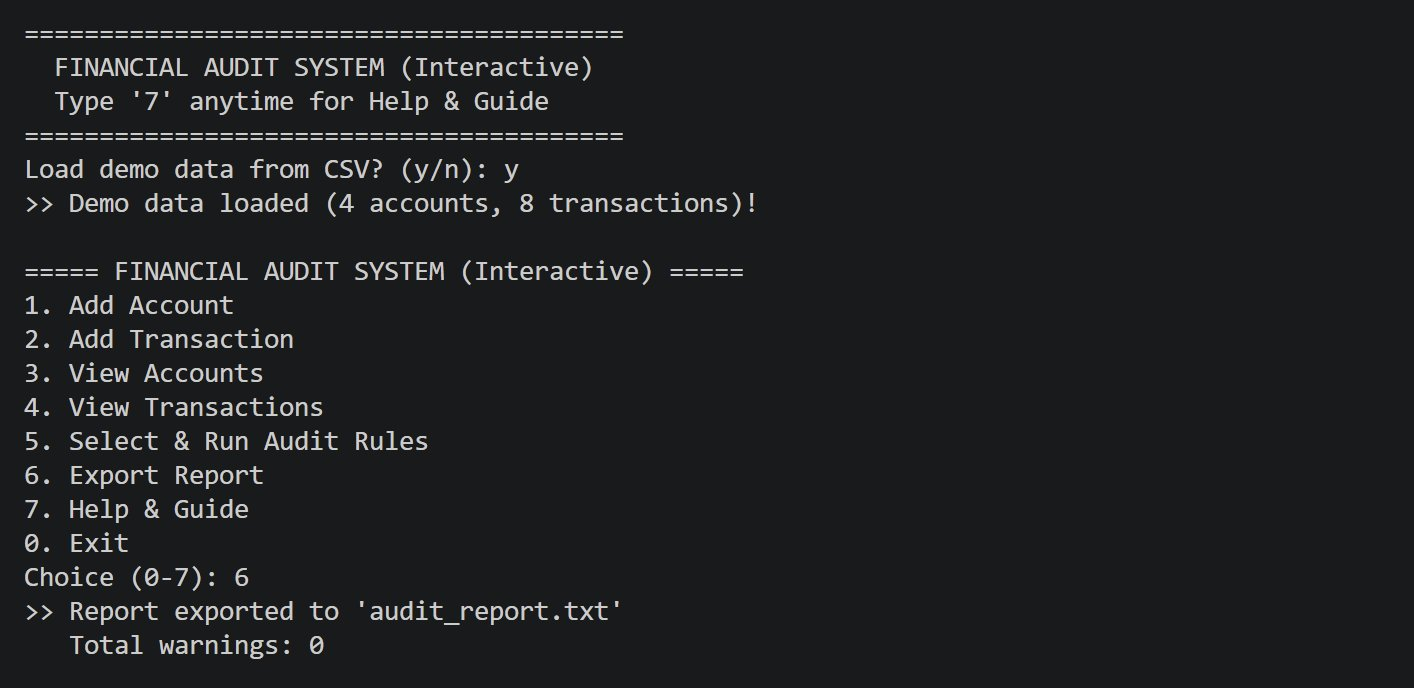
\includegraphics[width=\textwidth]{menu.png}
        \caption{The interactive menu of the system and the report-export operation.}
        \label{fig:menu}
    \end{figure}

    \subsection{Running the Audit}
    After loading the sample data set of 4 accounts and 8 transactions, the user can select any combination of audit rules to run. Figure~\ref{fig:audit_output} illustrates the case where the \texttt{GeoAnomalyRule} is selected: the system correctly detects transaction \texttt{TX007} originating from Iran -- a high-risk country -- and flags it with a \texttt{MEDIUM} severity level. Each rule can be enabled independently, and selecting all four rules yields the full set of warnings.

    \begin{figure}[H]
        \centering
        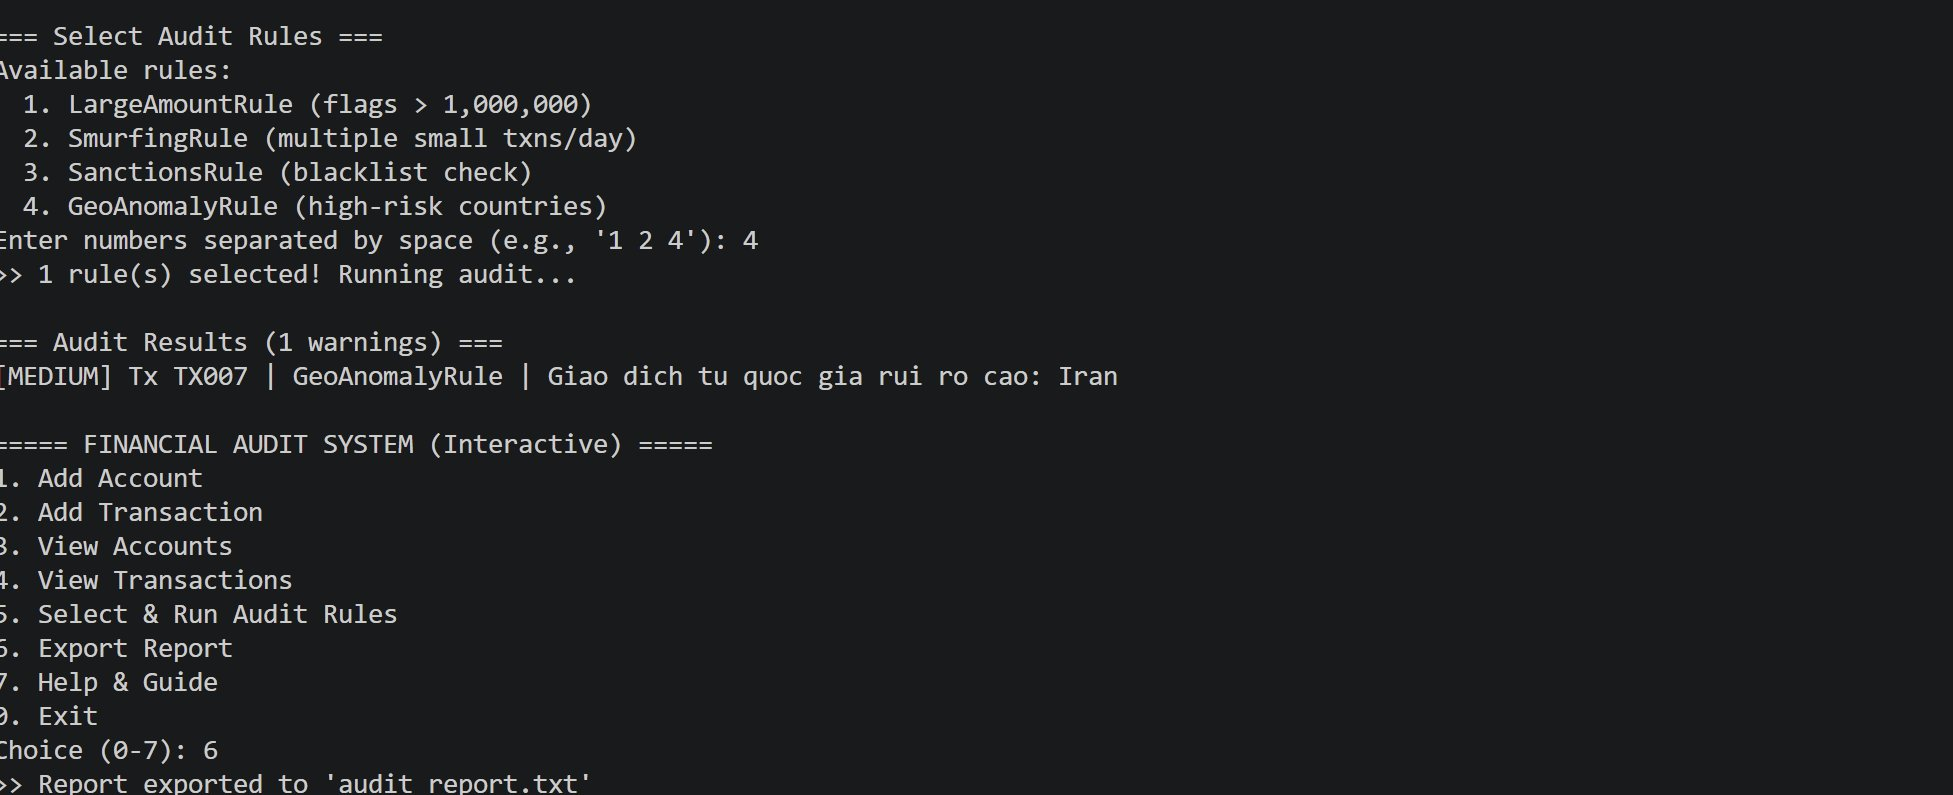
\includegraphics[width=\textwidth]{audit_output.png}
        \caption{Selecting an audit rule and the corresponding detection result.}
        \label{fig:audit_output}
    \end{figure}

    \subsection{Exported Report File}
    The audit result is also exported to a plain-text file \texttt{audit\_report.txt}, fulfilling the requirement of storing data in files. Figure~\ref{fig:report_output} shows the content of the exported report, including the total number of warnings and a detailed description of each violation.

    \begin{figure}[H]
        \centering
        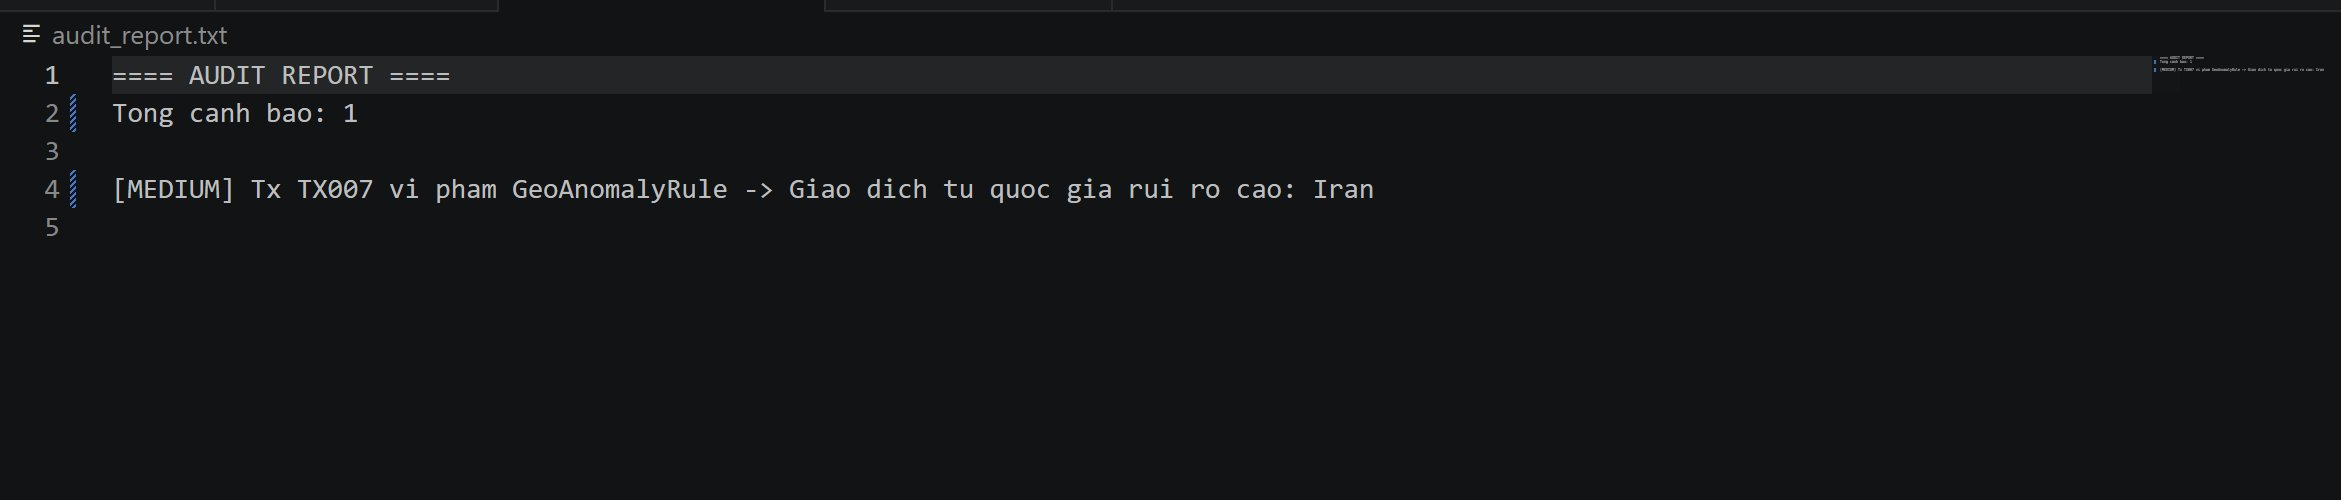
\includegraphics[width=\textwidth]{report_output.png}
        \caption{Content of the exported audit report file.}
        \label{fig:report_output}
    \end{figure}

    \subsection{Memory Management Verification}
    To prove that the program does not leak memory, the group recompiled it with the \texttt{-fsanitize=address,leak} flag and ran it. The AddressSanitizer tool confirmed that no memory leaks were detected, validating the correctness of the Rule of Five and the Virtual Constructor idiom.

\section{Division of Work}
    The group applies a feature-based Git branching model. The four members take charge of the four architectural modules; each member ``owns'' one OOP principle to present, ensuring no overlap and that every member participates in coding. The details are presented in Table~\ref{tab:phancong}.

    \begin{table}[H]
        \centering
        \caption{Division of work and responsibilities of members}
        \label{tab:phancong}
        \begin{tabular}{|l|p{4cm}|p{3.8cm}|}
            \hline
            \textbf{Member} & \textbf{Files in charge} & \textbf{Key principle} \\ \hline
            Mai Nam Khanh \textit{(Leader)} & \texttt{DataManagement}, \texttt{AuditEngine}, \texttt{FileManager}, \texttt{ConsoleUI} & Memory management, Aggregation, I/O \\ \hline
            Hoang Le Anh Duc & \texttt{Account.h/.cpp} & Inheritance, Encapsulation \\ \hline
            Vu Duy Tuan & \texttt{Transaction.h/.cpp}, \texttt{Common.h} & Multiple inheritance, Composition \\ \hline
            Pham Duc Tri & \texttt{AuditRule.h/.cpp} & Abstraction, Polymorphism \\ \hline
        \end{tabular}
    \end{table}


\chapter*{Conclusion}
\addcontentsline{toc}{chapter}{Conclusion}
\subsection*{Achieved Results}
Through the process of researching, designing, and implementing the topic ``Design and Implementation of a Financial Transaction Management \& Audit System using Object-Oriented Programming'', the group has achieved the following concrete results:

\begin{itemize}
    \item Successfully built a complete software system in C++ capable of managing accounts and transactions, and automatically detecting suspicious transactions based on an extensible set of audit rules.
    \item Fully and correctly applied the core principles of Object-Oriented Programming: abstraction, encapsulation, single and multiple inheritance, and polymorphism through dynamic dispatch.
    \item Applied advanced memory-management techniques in modern C++ (the Rule of Five and the Virtual Constructor idiom via \texttt{clone()}), ensuring the program is free of memory leaks, as verified using the AddressSanitizer tool.
    \item Designed a software architecture compliant with the SOLID principles, in particular the Single Responsibility Principle and the Open/Closed Principle, making the system easy to maintain and extend.
\end{itemize}

\subsection*{Future Work}
Building on this foundation, the system can be extended in the following directions:
\begin{enumerate}
    \item Replace the \texttt{double} type used to represent monetary values with a smallest-unit integer type (\texttt{int64\_t} cents) or a dedicated \texttt{Money} class, to eliminate floating-point rounding errors -- a mandatory requirement in real-world financial systems.
    \item Integrate a relational database (MySQL, PostgreSQL) instead of CSV files to manage large data volumes and support complex queries.
    \item Add advanced machine-learning-based audit rules (behavioural anomaly detection) and extend the system to a graphical user interface or a web service.
\end{enumerate}

\bibliographystyle{plain}
\urlstyle{rm}
\renewcommand{\bibname}{References}
\bibliography{refs}

\end{document}
